\scanpage{19}
de Kostant. On a donc \unsure{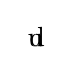
\begin{tikzpicture}[baseline=(ud.base)]\node[inner sep=0pt,anchor=base] (ud) at (0,0) {u};\node[inner sep=0pt,anchor=base] at (.025,0) {d};\end{tikzpicture}}\unsure{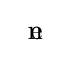
\begin{tikzpicture}[baseline=(ne.base)]\node[inner sep=0pt,anchor=base] (ne) at (0,0) {n};\node[inner sep=0pt,anchor=base] at (.015,0) {e};\end{tikzpicture}}s morphismes $f\handwritten{\unsure{\mathrel{\mapstochar\relbar}|\mapsto}}f\handwritten{\circ}i_o$ et $f\handwritten{\mapsto}f(u_o)$ de $\operatorname{Dyn}_c$ dans $\operatorname{ST}_c$ resp. $\operatorname{Un}_c$. D'autre part, Deligne nous fournit $\operatorname{Un}_c\handwritten{\to\underline{\varnothing}}_c$, et celui-ci peut aussi être défini par la commutativité du diagramme \handwritten{d'esp. homogènes}
% The two first cells of the overprinted word preserve u/d and n/e contours; order is uncertain.
\diagram{\begin{tikzpicture}
\node[anchor=north west,inner sep=0pt] at (0,0) {\begin{tikzcd}[ampersand replacement=\&,column sep=large,row sep=large]
\operatorname{ST}_c\handwritten{\simeq}(\operatorname{CL})_{c'} \handwritten{\arrow[d]}
\arrow[d,draw=gray!45,-,to path={([xshift=-.25ex,yshift=.45ex]\tikztotarget.north) .. controls +(0,-.65ex) and +(0,-.65ex) .. ([xshift=.25ex,yshift=.45ex]\tikztotarget.north)}]
\arrow[d,phantom,"{\unsure{}}" description,near end]
\& \operatorname{Dyn}_c \handwritten{\arrow[l]} \handwritten{\arrow[d]} \\
\handwritten{\underline{\varnothing}}_c\handwritten{\simeq}\operatorname{Par}_{c'} \& \operatorname{Un}_c\quad\text{.} \handwritten{\arrow[l]}
\end{tikzcd}};
\node[anchor=north west,inner sep=0pt] at (7.3,0) {\handwritten{\begin{tikzcd}[ampersand replacement=\&,column sep=small,row sep=small]
L \arrow[d] \& \unsure{\text{\begin{tikzpicture}[baseline=(zo.base)]\node[inner sep=0pt] (zo) at (0,0) {$Z_{\unsure{o|0}}$};\draw[line width=1.1pt] (-.04,.10) -- (-.04,-.17);\draw[line width=.8pt] (-.12,-.10) -- (.07,-.10);\end{tikzpicture}}} \arrow[l] \arrow[d] \\
P \& \unsure{\mathfrak{z}|z|Z}(\unsure{\mathord{\cdot}}e) \arrow[l]
\end{tikzcd}}};
\end{tikzpicture}}
% The extra strokes on the small square's Z are retained graphically; their predecessor and order are not established.

Pour qu'il existe un point rationnel de \deleted{$\operatorname{Dyn}_c$, ou ce qui revient au même} $\handwritten{\underline{\varnothing}}_c\handwritten{\simeq}\operatorname{Par}_{c'}$, il faut (et suffit) qu'il en existe un de $\operatorname{Dy}\unsure{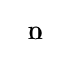
\begin{tikzpicture}[baseline=(n.base)]\node[inner sep=0pt] (n) {$\mathrm n$};\node[inner sep=0pt] at ([xshift=.02em,yshift=-.02ex]n.center) {$\mathrm o$};\end{tikzpicture}}_c$ \deleted{i.e. que $G$ soit quasi-déployé\unsure{;}}\inserted{\handwritten{(i.e.,, si $Z_o=e$, que $G$ est quasi-déployé)}}: en effet, $P$ étant choisi, \deleted{\unsure{les|des} $i$}\begin{tikzpicture}[baseline=-.1ex]\draw[line width=.3pt](0,0)--(.48em,.8ex);\draw[line width=.3pt](0,.8ex)--(.48em,0);\end{tikzpicture} on peut en choisir un \deleted{point rationnel}\begin{tikzpicture}[baseline=-.1ex]\draw[line width=.3pt](0,0)--(.48em,.8ex);\draw[line width=.3pt](0,.8ex)--(.48em,0);\end{tikzpicture} sous-groupe de Lévi
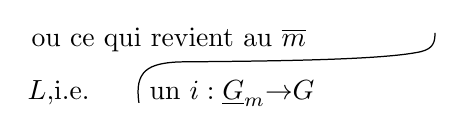
\begin{tikzpicture}[baseline=(levi.base)]
\node[anchor=base west,inner sep=0pt] (levi) at (0,0) {$L$,\deleted{i.e}.};
\node[anchor=base west,inner sep=0pt] at (1.55,0) {un $i:\underline{G}_m\handwritten{\to}G$};
\node[anchor=base west,inner sep=0pt] at (.05,.68) {\inserted{\handwritten{ou ce qui revient au $\overline{m}$}}};
\draw[line width=.45pt] (1.42,-.04) .. controls (1.36,.37) and (1.54,.46) .. (1.92,.48) .. controls (3.00,.49) and (4.50,.50) .. (5.00,.61) .. controls (5.16,.65) and (5.18,.73) .. (5.18,.85);
\end{tikzpicture}
dans la classe $c$,définissant $P$, et alors les $u=\exp(e)$ qui \deleted{\unsure{aue|aux}} s'adaptent à $i$ forment un ouvert dense de $\handwritten{\unsure{\mathfrak{g}|\mathscr{G}}(\unsure{2|\underline{2}})}$, qui \deleted{est donc non vide} a donc un point rationnel. On voit donc que pour certaines classes de paraboliques (qu'on pourrait appeler les paraboliques de
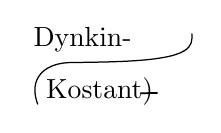
\begin{tikzpicture}[baseline=(kostant.base)]
\node[anchor=base west,inner sep=0pt] (kostant) at (.16,0) {Kostant\unsure{)}};
\draw[line width=.65pt] ([xshift=-.48em,yshift=.4ex]kostant.base east)--++(.62em,.03ex);
\node[anchor=base west,inner sep=0pt] at (0,.65) {\inserted{Dynkin-}};
\draw[line width=.45pt] (.06,-.08) .. controls (-.06,.24) and (.13,.43) .. (.44,.45) .. controls (.90,.46) and (1.68,.45) .. (1.92,.60) .. controls (2.02,.66) and (2.02,.73) .. (2.02,.82);
\end{tikzpicture}
l'existence d'un parabolique de cette classe rationnel sur $k$ implique déjà que $G$ est quasi-déployé. (NB Quand $G$ n'est pas une forme intérieure, il faut faire attention cependant de vérifier d'abord que la classe $c'$ de $P$ provient bien d'un $c$ de Dynkin \uline{invariant par} $\handwritten{\Gamma}$, et il n'est pas clair que cette propriété
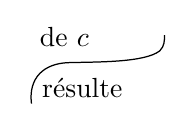
\begin{tikzpicture}[baseline=(resulte.base)]
\node[anchor=base west,inner sep=0pt] (resulte) at (.15,0) {résulte};
\node[anchor=base west,inner sep=0pt] at (.12,.64) {\inserted{de $c$}};
\draw[line width=.45pt] (.02,-.08) .. controls (-.02,.25) and (.18,.43) .. (.49,.44) .. controls (.86,.45) and (1.46,.44) .. (1.65,.59) .. controls (1.71,.65) and (1.71,.72) .. (1.71,.79);
\end{tikzpicture}
du fait que $c'$ est invariant\unsure{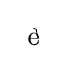
\begin{tikzpicture}[baseline=(endletter.base)]\node[inner sep=0pt,anchor=base] (endletter) at (0,0) {e};\draw[line width=.3pt] ([xshift=.37em,yshift=.82ex]endletter.base west)--++(-.04em,.5ex)--++(-.1em,.12ex);\draw[line width=.25pt] ([xshift=.40em,yshift=.45ex]endletter.base west) .. controls +(.02em,-.25ex) and +(.12em,-.02ex) .. ([xshift=.23em,yshift=.05ex]endletter.base west);\end{tikzpicture}} par $\handwritten{\Gamma}$, faute de savoir si $c\handwritten{\mapsto}c'$ est injectif sur les classes de Dynkin). \handwritten{(}On notera aussi que l'argument donné \unsure{
\begin{tikzpicture}[baseline=(m.base)]\node[inner sep=0pt] (m) {m};\node[inner sep=0pt] at ([xshift=.01em,yshift=-.01ex]m.center) {p};\end{tikzpicture}}arche également sur un anneau semi-local (de car. nulle jusqu'à nouvel ordre).\handwritten{)}
\margin{\handwritten{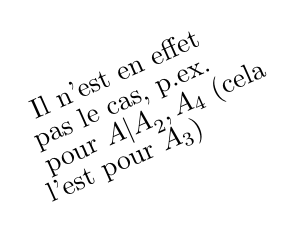
\begin{tikzpicture}[rotate=24,transform shape]
\node[anchor=base west,inner sep=0pt] at (0,0) {Il n'est en effet};
\node[anchor=base west,inner sep=0pt] at (-.12,-.35) {pas le cas, p.ex.};
\node[anchor=base west,inner sep=0pt] at (-.12,-.70) {pour $\unsure{A|\mathbb{A}}_2,A_4$ (cela};
\node[anchor=base west,inner sep=0pt] at (-.24,-1.05) {l'est pour $A_3$)};
\end{tikzpicture}}}
% margin note written slanted, rising to the right
Ceci montre l'intérêt, pour \unsure{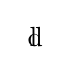
\begin{tikzpicture}[baseline=(ld.base)]\node[inner sep=0pt,anchor=base] (ld) at (0,0) {l};\node[inner sep=0pt,anchor=base] at (.025,0) {d};\end{tikzpicture}}es questions arithmétiques, de déterminer exactement les
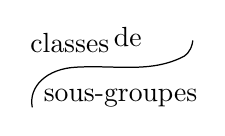
\begin{tikzpicture}[baseline=(sous.base)]
\node[anchor=base west,inner sep=0pt] (sous) at (.17,0) {sous-groupes};
\node[anchor=base west,inner sep=0pt] at (0,.63) {\inserted{classes\,\raisebox{.45ex}{\handwritten{de}}}};
\draw[line width=.45pt] (.03,-.07) .. controls (-.02,.20) and (.22,.42) .. (.58,.44) .. controls (1.10,.47) and (1.54,.36) .. (1.96,.58) .. controls (2.04,.64) and (2.06,.71) .. (2.07,.78);
\end{tikzpicture}
parab\handwritten{\unsure{\begin{tikzpicture}[baseline=-.2ex]\draw[line width=.7pt] (0,-.025) -- (.25,.045);\draw[line width=.2pt,gray!50] (.025,.07)--(.25,.17);\end{tikzpicture}}}oliques de Dynkin-Kostant des divers groupes simples, et de voir si: leur stabilisateur dans $\operatorname{Autext}(G_o)$ est le même que celui des $c$ de Dynkin correspondants, et pas str. plus grand.
% The d/l overprint is retained without assigning a chronological order.
% The diagonal joining stroke in paraboliques is drawn, not silently treated as a lexical hyphen.

On notera cependant que si une filtration du foncteur \deleted{fib} oubli peut être définie par un élément unipotent, la classe de conjugaison de ce der%
% Source has a line-end hyphen after der; the word continues beyond this scan.
% archive sheet number: 18
